\documentclass[aspectratio=169,10pt]{beamer}

\usepackage[T1]{fontenc}
\usepackage[utf8]{inputenc}
\usepackage{lmodern}
\usepackage{microtype}
\usepackage{amsmath}
\usepackage{booktabs}
\usepackage{array}
\usepackage{graphicx}
\usepackage{fancyvrb}
\usepackage{pgfplots}
\pgfplotsset{compat=1.18}
\usetikzlibrary{arrows.meta,positioning,calc}

\graphicspath{{./}{docs/slides/}}

% Visual system reused from lm_idnet_project_presentation.tex.
\definecolor{burgundy}{HTML}{990000}
\definecolor{darkburgundy}{HTML}{59000E}
\definecolor{dustyrose}{HTML}{D1545B}
\definecolor{palerose}{HTML}{E5D5D6}
\definecolor{paper}{HTML}{F7F6F2}
\definecolor{softgray}{HTML}{ECEAE7}
\definecolor{midgray}{HTML}{77736F}
\definecolor{charcoal}{HTML}{434343}
\definecolor{ink}{HTML}{111111}

\setbeamercolor{normal text}{fg=ink,bg=paper}
\setbeamercolor{structure}{fg=burgundy}
\setbeamercolor{frametitle}{fg=ink,bg=paper}
\setbeamercolor{title}{fg=white}
\setbeamercolor{subtitle}{fg=palerose}
\setbeamercolor{block title}{fg=white,bg=darkburgundy}
\setbeamercolor{block body}{fg=ink,bg=softgray}
\setbeamercolor{exampleblock title}{fg=white,bg=burgundy}
\setbeamercolor{exampleblock body}{fg=ink,bg=palerose!62!paper}
\setbeamercolor{alertblock title}{fg=white,bg=charcoal}
\setbeamercolor{alertblock body}{fg=ink,bg=softgray}
\setbeamercolor{ascii body}{fg=palerose,bg=ink}

\setbeamerfont{title}{series=\bfseries,size=\Huge}
\setbeamerfont{subtitle}{size=\large}
\setbeamerfont{frametitle}{series=\bfseries,size=\Large}
\setbeamerfont{footline}{size=\scriptsize}
\setbeamertemplate{navigation symbols}{}
\setbeamertemplate{itemize item}{\color{burgundy}$\blacktriangleright$}
\setbeamertemplate{itemize subitem}{\color{dustyrose}$\bullet$}
\setbeamertemplate{caption}{\raggedright\insertcaption\par}
\setbeamertemplate{frametitle}{%
  \vspace{0.18cm}%
  \hspace{0.42cm}\insertframetitle\par
  \vspace{-0.12cm}%
  \hspace{0.42cm}{\color{burgundy}\rule{14.95cm}{0.6pt}}%
}
\setbeamertemplate{footline}{%
  \leavevmode%
  \hbox{%
    \begin{beamercolorbox}[wd=.83\paperwidth,ht=2.8ex,dp=1.1ex,leftskip=1em]{author in head/foot}%
      \color{charcoal}\insertsectionhead
    \end{beamercolorbox}%
    \begin{beamercolorbox}[wd=.17\paperwidth,ht=2.8ex,dp=1.1ex,rightskip=1em plus1fil]{date in head/foot}%
      \color{burgundy}\hfill\insertframenumber
    \end{beamercolorbox}%
  }%
}

\setlength{\tabcolsep}{5pt}
\renewcommand{\arraystretch}{1.18}

\newcommand{\workingbadge}{%
  \colorbox{burgundy!13}{\color{darkburgundy}\scriptsize\bfseries\strut WORKING}}
\newcommand{\openbadge}{%
  \colorbox{dustyrose!18}{\color{burgundy}\scriptsize\bfseries\strut OPEN}}
\DefineVerbatimEnvironment{asciiart}{Verbatim}{
  fontsize=\small,
  baselinestretch=0.90,
  frame=none,
  fillcolor=\color{softgray},
  formatcom=\color{darkburgundy}
}

\tikzset{
  flowbox/.style={
    draw=burgundy,
    line width=0.7pt,
    rounded corners=1pt,
    fill=paper,
    minimum height=1.0cm,
    text width=2.35cm,
    align=center,
    font=\small\bfseries
  },
  smallflow/.style={
    draw=charcoal,
    rounded corners=1pt,
    fill=softgray,
    minimum height=0.78cm,
    text width=1.85cm,
    align=center,
    font=\scriptsize\bfseries
  },
  flowarrow/.style={-{Latex[length=2.2mm]},thick,draw=charcoal}
}

\title[LM-Backend]{LM-Backend Presentation}
\subtitle{Adaptive Dirichlet--Multinomial Anomaly Detection for IoT Traffic}
\author{Fatemeh Mahvari}
\institute{Supervisor: Professor Mauro Migliardi}
\date{28 September 2026}

\begin{document}

% 0:30
\begin{frame}[plain]
\begin{tikzpicture}[remember picture,overlay]
  \fill[ink] (current page.south west) rectangle (current page.north east);
  \fill[darkburgundy]
    (current page.south west) rectangle
    ([xshift=.64\paperwidth]current page.north west);
  \fill[burgundy,opacity=.28]
    ([xshift=.58\paperwidth]current page.south west) rectangle
    ([xshift=.67\paperwidth]current page.north west);
  \node[anchor=east,inner sep=0pt] (detector)
    at ([xshift=-0.42cm]current page.east)
    {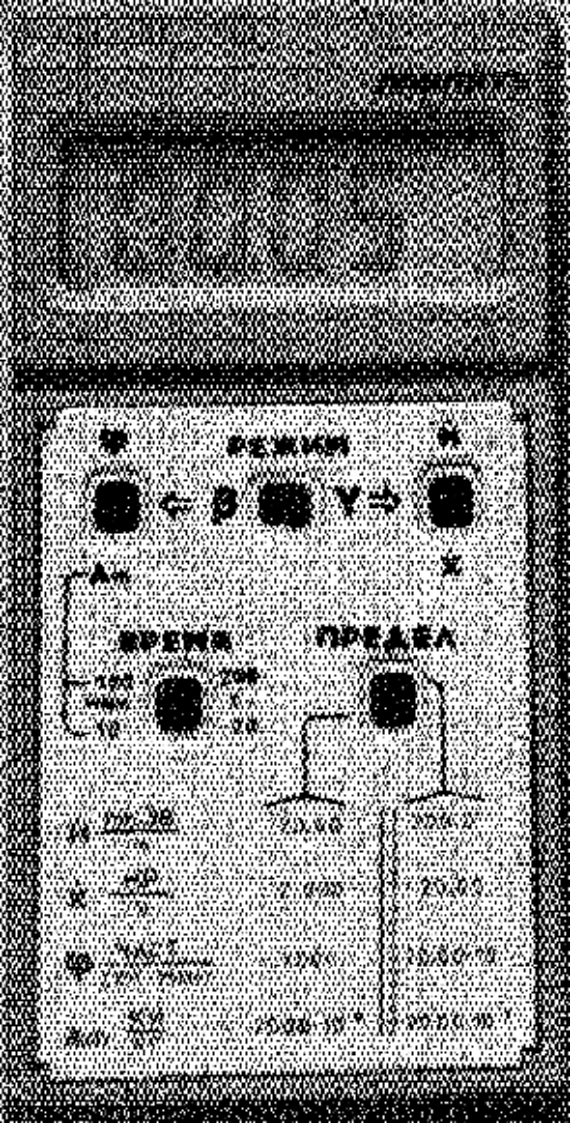
\includegraphics[height=.91\paperheight]{anomaly_detector.png}};
  \draw[palerose,line width=0.8pt]
    ([xshift=-0.10cm,yshift=0.10cm]detector.north west) rectangle
    ([xshift=0.10cm,yshift=-0.10cm]detector.south east);
  \draw[dustyrose,line width=1.1pt]
    ([xshift=-0.28cm]detector.center) -- ([xshift=0.28cm]detector.center);
  \draw[dustyrose,line width=1.1pt]
    ([yshift=-0.28cm]detector.center) -- ([yshift=0.28cm]detector.center);
  \node[anchor=west,text width=.53\paperwidth]
    at ([xshift=.70cm,yshift=1.05cm]current page.west)
    {\color{white}\fontsize{26}{29}\selectfont\bfseries
     LM-Backend\\Presentation};
  \node[anchor=west,text width=.51\paperwidth]
    at ([xshift=.72cm,yshift=-.48cm]current page.west)
    {\color{palerose}\large Adaptive Dirichlet--Multinomial\\
     Anomaly Detection for IoT Traffic};
  \node[anchor=west]
    at ([xshift=.72cm,yshift=-1.42cm]current page.west)
    {\color{white!82}\ttfamily\small [ COUNT / MODEL / DETECT / ADAPT ]};
  \node[anchor=west,text width=.50\paperwidth]
    at ([xshift=.72cm,yshift=-2.35cm]current page.west)
    {\color{palerose!90}\small Working system, experimental evidence,\\
     and the route to a defensible final evaluation};
  \node[anchor=south west,text width=.53\paperwidth]
    at ([xshift=.72cm,yshift=.40cm]current page.south west)
    {\color{white}\small\bfseries Fatemeh Mahvari\\[-0.02cm]
     \color{palerose!90}\scriptsize Supervisor: Professor Mauro Migliardi
     \quad // \quad 28 September 2026};
  \node[anchor=south east,fill=ink,fill opacity=.82,text opacity=1,
        inner xsep=3pt,inner ysep=2pt]
    at ([xshift=-.06cm,yshift=.06cm]detector.south east)
    {\color{palerose!85}\tiny REFERENCE IMAGE // PRYPIAT DETECTOR};
  \node[anchor=south east]
    at ([xshift=-.18cm,yshift=.15cm]current page.south east)
    {\color{palerose}\scriptsize\insertframenumber};
\end{tikzpicture}
\end{frame}

\section{Project Context}

% 1:00
\begin{frame}{Presentation map}
\begin{columns}[T,onlytextwidth]
\column{0.48\textwidth}
\begin{block}{0 // Project context}
Goal, pipeline, current development evidence, and the role of LM.
\end{block}
\begin{block}{I // Fitted \(\psi\)}
The dispersion parameter, fitted values, and the baseline paper's threshold.
\end{block}

\column{0.48\textwidth}
\begin{block}{II // Row-wise backend}
Why windows remain separate and how the project adapted the scalar LM code.
\end{block}
\begin{block}{III // Evidence}
Timing boundaries, runtime results, optimization, and numerical agreement.
\end{block}
\begin{exampleblock}{Conclusion}
What the measurements support---and what they do not.
\end{exampleblock}
\end{columns}
\end{frame}

% 1:30
\begin{frame}{Project context: goal, pipeline, and current result}
\begin{columns}[T,onlytextwidth]
\column{0.53\textwidth}
LM-IDNet learns one device's normal traffic without attack examples during
training, then flags later windows that are unlikely under that model.

\vspace{0.35cm}
\centering
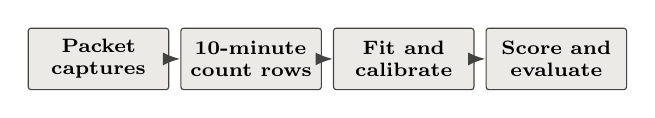
\begin{tikzpicture}[
  node distance=0.14cm,
  smallflow/.append style={text width=1.55cm}
]
\node[smallflow] (pcap) {Packet\\captures};
\node[smallflow,right=of pcap] (window) {10-minute\\count rows};
\node[smallflow,right=of window] (fit) {Fit and\\calibrate};
\node[smallflow,right=of fit] (score) {Score and\\evaluate};
\draw[flowarrow] (pcap) -- (window);
\draw[flowarrow] (window) -- (fit);
\draw[flowarrow] (fit) -- (score);
\end{tikzpicture}

\vspace{0.45cm}
\begin{itemize}
  \item Counts: TCP, ordinary UDP, SSDP, and ARP.
  \item Model: Dirichlet--multinomial normal behaviour.
  \item Decision: separately calibrated lower-tail likelihood threshold.
  \item Labels: used only after scoring for evaluation.
\end{itemize}

\column{0.43\textwidth}
\begin{block}{Labelled development F1}
\centering
\small
\begin{tabular}{@{}lrr@{}}
\toprule
& Static & Periodic refit \\
\midrule
Chromecast & 61.22\% & 80.70\% \\
Samsung & 78.69\% & 77.31\% \\
\bottomrule
\end{tabular}
\end{block}

\end{columns}
\end{frame}

% 1:00
\begin{frame}{Where the LM backend fits}
\centering
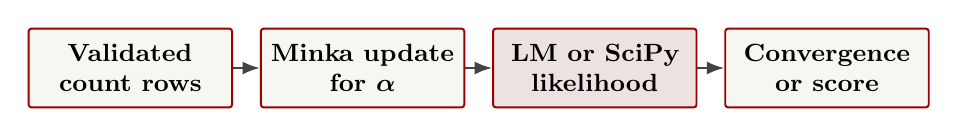
\begin{tikzpicture}[node distance=0.34cm]
\node[flowbox] (rows) {Validated\\count rows};
\node[flowbox,right=of rows] (minka) {Minka update\\for $\boldsymbol{\alpha}$};
\node[flowbox,right=of minka,fill=palerose!62!paper] (lm) {LM or SciPy\\likelihood};
\node[flowbox,right=of lm] (decision) {Convergence\\or score};
\draw[flowarrow] (rows) -- (minka);
\draw[flowarrow] (minka) -- (lm);
\draw[flowarrow] (lm) -- (decision);
\end{tikzpicture}

\vspace{0.60cm}
\begin{columns}[T,onlytextwidth]
\column{0.47\textwidth}
\begin{exampleblock}{LM does}
Evaluate close log-Gamma differences inside the Dirichlet--multinomial
likelihood, with explicit numerical error control.
\end{exampleblock}

\column{0.47\textwidth}
\begin{alertblock}{LM does not}
Choose the traffic representation, update alpha, derive \(\psi\), define the
paper's cutoff, set the anomaly threshold, or make an unchanged detector
statistically better.
\end{alertblock}
\end{columns}
\end{frame}

\section{Fitted \texorpdfstring{\(\psi\)}{psi} and the Data}

% 1:15
\begin{frame}{The backend receives one row per window}
\begin{columns}[c,onlytextwidth]
\column{0.43\textwidth}
\[
\mathbf{x}_r=
(x_{r,\mathrm{TCP}},x_{r,\mathrm{UDP}},
x_{r,\mathrm{SSDP}},x_{r,\mathrm{ARP}})
\]
\begin{itemize}
  \item SSDP is separated from ordinary UDP.
  \item Silent observed windows are zero rows.
  \item Missing capture coverage is excluded.
\end{itemize}

\column{0.53\textwidth}
\centering
\small
\begin{tabular}{@{}lrrrr@{}}
\toprule
Dataset & Days & Windows & Silent & Attack-labelled \\
\midrule
D-Link camera & 12 & 1,692 & 0 & -- \\
Chromecast & 17 & 2,349 & 187 & 38 \\
Samsung camera & 12 & 1,645 & 49 & 82 \\
\bottomrule
\end{tabular}

\vspace{0.45cm}
Since D-Link is unlabelled, it is used only to benchmark the LM algorithm, not
in the end-to-end detector pipeline.
\end{columns}

\vspace{0.30cm}
{\scriptsize
\textbf{Dataset sources}\par
UNSW Chromecast and Samsung camera:
\href{https://iotanalytics.unsw.edu.au/attack-data.html}{\color{burgundy}\nolinkurl{https://iotanalytics.unsw.edu.au/attack-data.html}}\par
D-Link Camera 5:
\href{https://data.mendeley.com/datasets/84cc8grtkt/1}{\color{burgundy}\nolinkurl{https://data.mendeley.com/datasets/84cc8grtkt/1}}
}
\end{frame}

% 1:30
\begin{frame}{The dispersion parameter and the numerical regime}
\begin{columns}[T,onlytextwidth]
\column{0.49\textwidth}
\begin{block}{Dirichlet--multinomial model}
The protocol-probability vector may vary between windows. This permits more
row-to-row variation than a fixed-probability Multinomial model.
\[
A=\sum_k\alpha_k,
\qquad \psi=\frac{1}{A}
\]
The project reports $\psi$ directly as the fitted Dirichlet--multinomial
dispersion parameter throughout the comparison.
\end{block}

\column{0.47\textwidth}
\begin{exampleblock}{LM numerical regime}
LM accepts positive $\boldsymbol{\alpha}$ and the corresponding $\psi$, then
evaluates the same likelihood as the reference backend. The paper's cutoff is
not an LM precondition.
\end{exampleblock}

\begin{alertblock}{Why small $\psi$ matters}
Smaller $\psi$ means larger concentration and a greater chance that subtracting
large, nearby log-Gamma values will lose precision.
\end{alertblock}
\end{columns}
\end{frame}

% 1:15
\begin{frame}{Baseline paper and its empirical rule}
\begin{block}{Main experimental baseline}
\emph{Modeling and Forecasting Overdispersed IoT Data Using an Efficient and
Accurate Computation of the Dirichlet Multinomial Distribution}\par
\smallskip
S. Al-Haj Baddar, A. Languasco, and M. Migliardi
\end{block}

\begin{columns}[T,onlytextwidth]
\column{0.47\textwidth}
\begin{itemize}
  \item D-Link Camera 5 traffic
  \item Ten-minute, four-protocol vectors
  \item Dirichlet--multinomial fitting
  \item LM comparison and forecasting
\end{itemize}

\column{0.49\textwidth}
\begin{alertblock}{Paper-defined threshold: $\psi<0.05$}
The paper defines a dataset as overdispersed when its fitted $\psi$ is below
0.05. Numerical failure is not triggered at that exact line: its likelihood
increases progressively as $\psi$ becomes smaller.
\end{alertblock}
\end{columns}
\end{frame}

% 1:30
\begin{frame}{Aggregate fitted \texorpdfstring{$\psi$}{psi}: training versus all days}
\begin{columns}[c,onlytextwidth]
\column{0.68\textwidth}
\centering
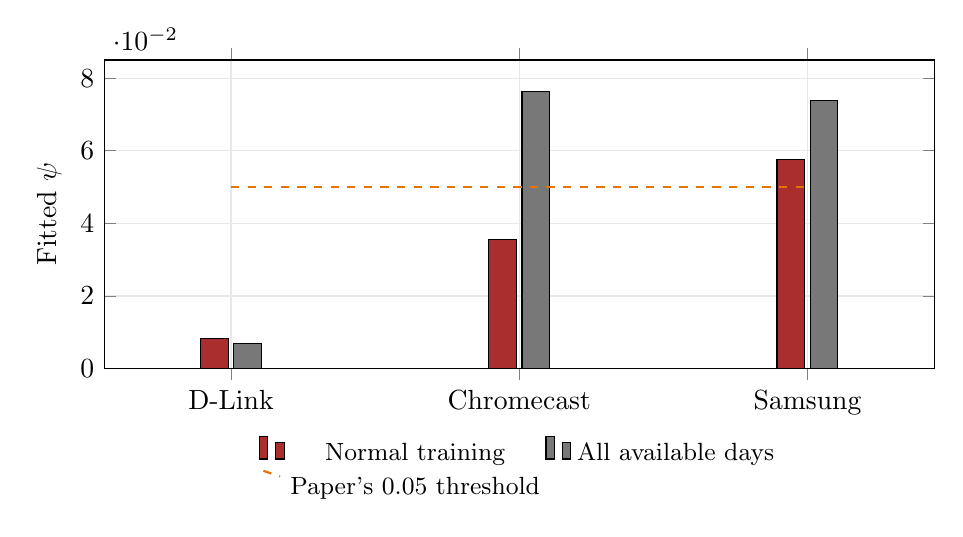
\begin{tikzpicture}
\begin{axis}[
  ybar,
  bar width=10pt,
  width=\linewidth,
  height=5.5cm,
  ymin=0,
  ymax=0.085,
  ylabel={Fitted $\psi$},
  symbolic x coords={D-Link,Chromecast,Samsung},
  xtick=data,
  enlarge x limits=0.22,
  grid=major,
  grid style={gray!18},
  legend style={font=\small,draw=none,at={(0.5,-0.20)},anchor=north,legend columns=2},
]
\addplot[fill=burgundy!82] coordinates {
  (D-Link,0.008182) (Chromecast,0.035589) (Samsung,0.057491)
};
\addlegendentry{Normal training}
\addplot[fill=charcoal!72] coordinates {
  (D-Link,0.006833) (Chromecast,0.076318) (Samsung,0.073784)
};
\addlegendentry{All available days}
\addplot[orange!90!black,dashed,thick,sharp plot] coordinates {
  (D-Link,0.05) (Chromecast,0.05) (Samsung,0.05)
};
\addlegendentry{Paper's $0.05$ threshold}
\end{axis}
\end{tikzpicture}

\column{0.28\textwidth}
\begin{block}{Below $0.05$}
D-Link in both scopes and Chromecast in normal training satisfy the paper's
condition.
\end{block}

\begin{alertblock}{Read the scopes}
All-days fits mix partitions and include attack periods for the labelled
devices. D-Link has the smallest aggregate $\psi$ and the greatest numerical
risk among these fits.
\end{alertblock}
\end{columns}
\end{frame}

% 1:30
\begin{frame}{Day-to-day change is change in fitted
  \texorpdfstring{$\psi$}{psi}}
\small
\begin{columns}[c,onlytextwidth]
\column{0.72\textwidth}
\centering
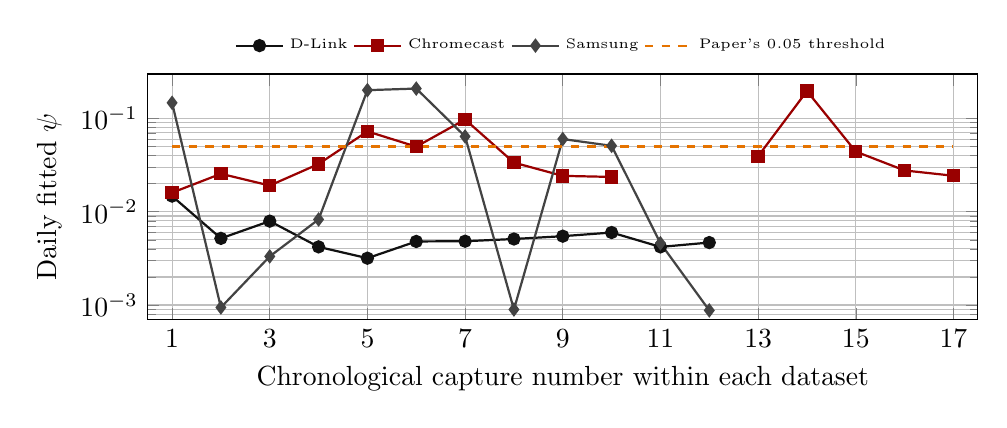
\begin{tikzpicture}
\begin{semilogyaxis}[
  width=\linewidth,
  height=4.7cm,
  xmin=0.5,
  xmax=17.5,
  ymin=0.0007,
  ymax=0.30,
  xlabel={Chronological capture number within each dataset},
  ylabel={Daily fitted $\psi$},
  xtick={1,3,5,7,9,11,13,15,17},
  grid=both,
  unbounded coords=jump,
  legend style={font=\tiny,draw=none,at={(0.5,1.04)},anchor=south,legend columns=4},
]
\addplot[ink,mark=*,thick] coordinates {
  (1,0.014719) (2,0.005184) (3,0.007931) (4,0.004202)
  (5,0.003178) (6,0.004805) (7,0.004832) (8,0.005104)
  (9,0.005472) (10,0.005989) (11,0.004198) (12,0.004676)
};
\addlegendentry{D-Link}
\addplot[burgundy,mark=square*,thick] coordinates {
  (1,0.016012) (2,0.025523) (3,0.019097) (4,0.032473)
  (5,0.072661) (6,0.049859) (7,0.097399) (8,0.033622)
  (9,0.024242) (10,0.023627) (11,nan) (12,nan)
  (13,0.039374) (14,0.196667) (15,0.044145) (16,0.027706)
  (17,0.024312)
};
\addlegendentry{Chromecast}
\addplot[charcoal,mark=diamond*,thick] coordinates {
  (1,0.147219) (2,0.000942) (3,0.003321) (4,0.008272)
  (5,0.201022) (6,0.209132) (7,0.064162) (8,0.000896)
  (9,0.060155) (10,0.050909) (11,0.004597) (12,0.000876)
};
\addlegendentry{Samsung}
\addplot[orange!90!black,dashed,thick,domain=1:17] {0.05};
\addlegendentry{Paper's $0.05$ threshold}
\end{semilogyaxis}
\end{tikzpicture}

\column{0.24\textwidth}
\scriptsize
\begin{block}{What is reported}
Each point is the day's fitted Dirichlet--multinomial dispersion parameter.
\end{block}
\begin{alertblock}{Numerical meaning}
The smaller the daily $\psi$, the greater the chance that conventional
log-Gamma likelihood evaluation loses precision. It is not a detector output.
\end{alertblock}
\end{columns}
\end{frame}

\section{The Row-Wise Backend}

% 1:20
\begin{frame}{Why the windows must remain separate}
\begin{columns}[c,onlytextwidth]
\column{0.44\textwidth}
\begin{block}{Two observed windows}
\[
\mathbf{x}_1=(2,0),
\qquad
\mathbf{x}_2=(1,1)
\]
Window 1 has no B; window 2 contains both A and B.
\end{block}

\begin{alertblock}{After pooling}
\[
\mathbf{x}_1+\mathbf{x}_2=(3,1)
\]
The total mixture remains, but the change between windows disappears.
\end{alertblock}

\column{0.52\textwidth}
\begin{exampleblock}{The detector's scientific question}
What protocol mixtures occur in individual windows, how much do those windows
vary, and is a later window plausible under the same device model?
\end{exampleblock}

\begin{itemize}
  \item Each row is one observation for fitting.
  \item Each later row is one anomaly decision.
  \item Pooling is suitable only for a different question: long-period total
  composition.
\end{itemize}
\end{columns}
\end{frame}

% 1:40
\begin{frame}{Evaluate rows, then add likelihoods}
For separate observations, probabilities multiply and log-likelihoods add:
\[
\ell_{\mathrm{rows}}(\boldsymbol{\alpha})
=\ell(\mathbf{x}_1;\boldsymbol{\alpha})
 +\ell(\mathbf{x}_2;\boldsymbol{\alpha}).
\]

\begin{columns}[T,onlytextwidth]
\column{0.48\textwidth}
\begin{exampleblock}{Row-wise objective}
\centering
$K((2,0);\boldsymbol{\alpha})+K((1,1);\boldsymbol{\alpha})$\\[0.18cm]
\Large $-2.89037$
\end{exampleblock}

\column{0.48\textwidth}
\begin{alertblock}{Pooled objective}
\centering
$K((3,1);\boldsymbol{\alpha})$\\[0.18cm]
\Large $-2.99573$
\end{alertblock}
\end{columns}

\vspace{0.25cm}
\small Here $\boldsymbol{\alpha}=(1,1)$. Neither number is inherently ``more
accurate'': they are different likelihoods for different statistical
questions. The project needs the row-wise one.
\end{frame}

% 1:30
\begin{frame}{Original capsule versus project objective}
\small
\begin{tabular}{>{\raggedright\arraybackslash}p{0.19\textwidth}
                >{\raggedright\arraybackslash}p{0.34\textwidth}
                >{\raggedright\arraybackslash}p{0.37\textwidth}}
\toprule
& Original LM-wrapped capsule & Production project \\
\midrule
Minka update & Uses the original rows & Uses the original rows \\
\addlinespace
Convergence likelihood & \texttt{find\_X} sums columns, then one scalar LM
call evaluates the pooled vector & Matrix interface evaluates every row, then
sums the returned likelihood values \\
\addlinespace
Calls per iteration & Old and candidate pooled likelihoods & One new row-wise
matrix likelihood; previous value is retained \\
\addlinespace
Meaning & One long-period composition vector & Separate time-window
observations under one shared model \\
\bottomrule
\end{tabular}

\vspace{0.45cm}
\begin{alertblock}{The distinction}
The original estimator does use rows in its update. The difference is the
likelihood objective used to decide convergence, not whether rows exist at all.
\end{alertblock}
\end{frame}

% 1:30
\begin{frame}{Project integration: preserve rows, reuse setup}
\centering
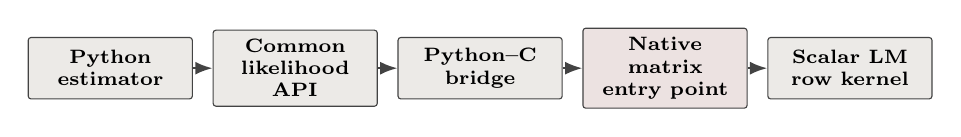
\begin{tikzpicture}[node distance=0.25cm]
\node[smallflow] (est) {Python\\estimator};
\node[smallflow,right=of est] (api) {Common\\likelihood API};
\node[smallflow,right=of api] (bridge) {Python--C\\bridge};
\node[smallflow,right=of bridge,fill=palerose!62!paper] (matrix) {Native matrix\\entry point};
\node[smallflow,right=of matrix] (scalar) {Scalar LM\\row kernel};
\draw[flowarrow] (est) -- (api);
\draw[flowarrow] (api) -- (bridge);
\draw[flowarrow] (bridge) -- (matrix);
\draw[flowarrow] (matrix) -- (scalar);
\end{tikzpicture}

\vspace{0.52cm}
\begin{columns}[T,onlytextwidth]
\column{0.47\textwidth}
\begin{block}{Earlier adapter}
For every row: prepare LM settings, validate, evaluate, release. Correct, but
alpha- and precision-dependent setup was repeated.
\end{block}

\column{0.47\textwidth}
\begin{exampleblock}{Current adapter}
Prepare shared settings once, validate and evaluate each row separately, sum
the values, then release the workspace once.
\end{exampleblock}
\end{columns}

\smallskip
\small Zero counts, file loading, allocation failures, dimensions, finite
results, memory ownership, and reproducible compilation remain checked.
\end{frame}

\section{Runtime and Numerical Evidence}

% 1:20
\begin{frame}{Four timers that must not be confused}
\scriptsize
\begin{tabular}{>{\bfseries}p{0.20\textwidth}p{0.36\textwidth}p{0.34\textwidth}}
\toprule
Measurement & Included & Excluded \\
\midrule
Complete model fit & Alpha initialization, initial likelihood, Minka updates,
iterative row-wise likelihoods, convergence checks & PCAP preprocessing, JSON
loading, backend construction, saving, calibration, scoring \\
\addlinespace
Training likelihood & One fixed-alpha call on the complete training matrix &
Initialization, updates, iterations, coefficient, file I/O \\
\addlinespace
Single-window score & Full log-probability for one non-silent row & Window
loading, threshold comparison, event output, evaluation \\
\addlinespace
Original printed time & Two pooled likelihood calls per Minka iteration &
Minka update, setup outside calls, data loading, total fit wall time \\
\bottomrule
\end{tabular}

\vspace{0.40cm}
{\color{burgundy}\bfseries
The reported ``complete model fit'' is not the complete command-line pipeline;
packet preprocessing is excluded.}
\end{frame}

% 1:45
\begin{frame}{Production runtime is workload-dependent}
\begin{columns}[c,onlytextwidth]
\column{0.75\textwidth}
\centering
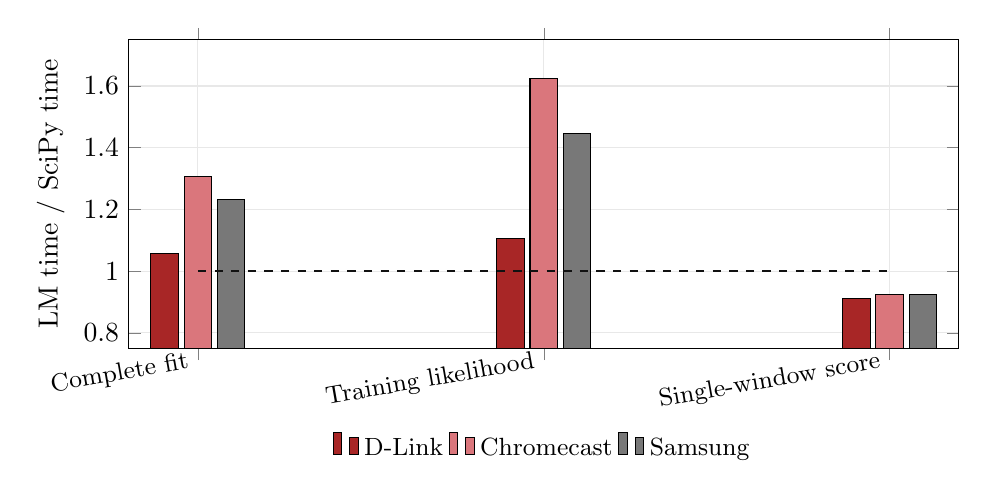
\begin{tikzpicture}
\begin{axis}[
  ybar,
  bar width=10pt,
  width=\linewidth,
  height=5.5cm,
  ymin=0.75,
  ymax=1.75,
  ylabel={LM time / SciPy time},
  symbolic x coords={fit,matrix,window},
  xtick=data,
  xticklabels={Complete fit,Training likelihood,Single-window score},
  x tick label style={font=\small,rotate=10,anchor=east},
  grid=major,
  grid style={gray!18},
  legend style={font=\small,draw=none,at={(0.5,-0.25)},anchor=north,legend columns=3},
]
\addplot[fill=burgundy!85] coordinates {(fit,1.058) (matrix,1.105) (window,0.910)};
\addlegendentry{D-Link}
\addplot[fill=dustyrose!80] coordinates {(fit,1.307) (matrix,1.625) (window,0.924)};
\addlegendentry{Chromecast}
\addplot[fill=charcoal!72] coordinates {(fit,1.232) (matrix,1.447) (window,0.923)};
\addlegendentry{Samsung}
\draw[ink,dashed,thick] (axis cs:fit,1) -- (axis cs:window,1);
\end{axis}
\end{tikzpicture}

\column{0.21\textwidth}
\begin{alertblock}{Matrix work}
LM is slower for the three large row-wise likelihoods and complete fits.
\end{alertblock}
\begin{exampleblock}{Online work}
LM is about 8--9\% faster for one complete single-window score.
\end{exampleblock}
\end{columns}
\end{frame}

% 1:00
\begin{frame}{Row-wise adapter optimization}
\centering
\begin{minipage}{0.68\textwidth}
\begin{exampleblock}{Before and after}
\centering
\small
\begin{tabular}{@{}lrr@{}}
\toprule
Operation & Earlier LM & Current LM \\
\midrule
846-row likelihood & 114.68 $\mu$s & 55.58 $\mu$s \\
Complete fit & 0.30410 s & 0.19486 s \\
\bottomrule
\end{tabular}

\medskip
\textbf{51.5\%} and \textbf{35.9\%} reductions, with identical row-wise
results across 1,000 stress matrices.
\end{exampleblock}
\end{minipage}
\end{frame}

% 1:45
\begin{frame}{Agreement now; protection near the boundary}
\begin{columns}[T,onlytextwidth]
\column{0.38\textwidth}
\begin{exampleblock}{D-Link production agreement}
\centering
\Large\textbf{0 / 270}\\[-0.04cm]
\small decision mismatches\\[0.30cm]
\scriptsize
\begin{tabular}{@{}lr@{}}
Relative alpha & $3.86\times10^{-7}$\\
Absolute score & $1.09\times10^{-5}$\\
Threshold & $2.89\times10^{-6}$
\end{tabular}
\end{exampleblock}

\column{0.58\textwidth}
\begin{block}{Absolute error against high precision}
\centering
\scriptsize
\begin{tabular}{@{}rrr@{}}
\toprule
$\psi$ & SciPy error & LM error \\
\midrule
$8.18\times10^{-3}$ & $3.07\times10^{-10}$ & $3.91\times10^{-10}$ \\
$10^{-8}$ & $2.50\times10^{-7}$ & $1.50\times10^{-8}$ \\
$10^{-10}$ & $2.83\times10^{-5}$ & $5.65\times10^{-8}$ \\
$10^{-12}$ & $2.02\times10^{-3}$ & $5.58\times10^{-5}$ \\
$10^{-14}$ & $3.37\times10^{-1}$ & $1.03\times10^{-3}$ \\
\bottomrule
\end{tabular}
\end{block}

\small On current data, both backends are accurate. LM's numerical advantage
becomes material at extremely small $\psi$, where cancellation grows.
\end{columns}
\end{frame}

\section{Conclusion}

% 1:30
\begin{frame}{Conclusion: the defensible LM-backend claim}
\small
\begin{columns}[T,onlytextwidth]
\column{0.57\textwidth}
\begin{enumerate}
  \item \textbf{$\psi$ is the reported dispersion parameter.}
  The paper's $0.05$ threshold is shown directly on the aggregate and daily
  values.
  \item \textbf{Rows are part of the detector's meaning.}
  Evaluating each window and then adding likelihoods preserves the variation
  that pooling removes.
  \item \textbf{The integration is validated, not universally faster.}
  Shared setup materially improved the row-wise adapter; LM is faster for the
  measured single-window score, while SciPy is faster for current matrix fits.
  \item \textbf{Numerical value depends on regime.}
  Current decisions agree, and LM provides stronger protection as $\psi$
  becomes smaller and conventional cancellation risk increases.
\end{enumerate}

\column{0.39\textwidth}
\begin{exampleblock}{One-sentence result}
The optimized native backend preserves the project's row-wise objective and
numerical decisions; its speed advantage is conditional on the operation and
calling architecture.
\end{exampleblock}

\begin{alertblock}{Claim boundary}
No end-to-end pipeline or edge-device speed claim has been made.
\end{alertblock}
\end{columns}
\end{frame}

\begin{frame}[fragile]{Questions and discussion}
\centering
\vspace{0.35cm}
{\Huge\color{burgundy}\textbf{Questions?}}

\vspace{0.75cm}
\begin{center}
\begin{minipage}{0.50\textwidth}
\begin{asciiart}
      .---------------------------------.
  ))  | DISPERSION / ROWS / RUNTIME     |  ((
      | STATUS: READY FOR DISCUSSION   |
      '---------------------------------'
\end{asciiart}
\end{minipage}
\end{center}
\end{frame}

\appendix
\section{Backup}

\begin{frame}{Backup: exact production runtimes}
\centering
\scriptsize
\begin{tabular}{llrrrr}
\toprule
Operation & Dataset & SciPy & LM & LM/SciPy & Difference \\
\midrule
Complete fit & D-Link & 180.59 ms & 191.04 ms & 1.058 & $+5.8\%$ \\
& Chromecast & 194.40 ms & 254.17 ms & 1.307 & $+30.7\%$ \\
& Samsung & 34.47 ms & 42.46 ms & 1.232 & $+23.2\%$ \\
\addlinespace
Matrix likelihood & D-Link & 49.79 $\mu$s & 55.02 $\mu$s & 1.105 & $+10.5\%$ \\
& Chromecast & 52.12 $\mu$s & 84.69 $\mu$s & 1.625 & $+62.5\%$ \\
& Samsung & 31.57 $\mu$s & 45.69 $\mu$s & 1.447 & $+44.7\%$ \\
\addlinespace
Single score & D-Link & 13.18 $\mu$s & 12.00 $\mu$s & 0.910 & $-9.0\%$ \\
& Chromecast & 13.22 $\mu$s & 12.22 $\mu$s & 0.924 & $-7.6\%$ \\
& Samsung & 13.20 $\mu$s & 12.18 $\mu$s & 0.923 & $-7.7\%$ \\
\bottomrule
\end{tabular}

\vspace{0.55cm}
Five complete fits per backend; warmed isolated calls measured in five batches.
Backend construction and one-time coefficient loading occurred before timing.
\end{frame}

\begin{frame}{Backup: fit workloads}
\centering
\small
\begin{tabular}{lrrrr}
\toprule
Dataset & Matrix & Iterations & Initial likelihood & Final likelihood \\
\midrule
D-Link & $846\times4$ & 1,882 & $-477{,}950.796$ & $-476{,}052.589$ \\
Chromecast & $867\times4$ & 1,950 & $-1{,}464{,}261.145$ & $-1{,}462{,}542.173$ \\
Samsung & $432\times4$ & 580 & $-191{,}965.774$ & $-191{,}562.039$ \\
\bottomrule
\end{tabular}

\vspace{0.60cm}
\begin{alertblock}{Interpretation}
Absolute fit times depend on both matrix size and iteration count. Likelihood
magnitudes also depend on the data and row count; they are convergence values,
not a ranking of device models.
\end{alertblock}
\end{frame}

\begin{frame}{Backup: native integration changes}
\begin{columns}[T,onlytextwidth]
\column{0.48\textwidth}
\begin{block}{Row-wise production path}
\begin{itemize}
  \item Matrix entry point over independent rows
  \item Shared alpha/precision setup once per matrix
  \item Same scalar LM numerical engine per row
  \item Previous convergence likelihood retained
\end{itemize}
\end{block}

\column{0.48\textwidth}
\begin{block}{Safety and operation}
\begin{itemize}
  \item Exact zero-count identity
  \item Checked dimensions, tables, and allocations
  \item Native errors returned to Python
  \item Explicit workspace release
  \item Reproducible shared-library rebuild
\end{itemize}
\end{block}
\end{columns}

\begin{alertblock}{Preserved reference}
The professor's files under \texttt{lm-algorithm/code/} remain unchanged; the
application-facing implementation lives in the project's native runtime copy.
\end{alertblock}
\end{frame}

\end{document}
